\chapter{El teorema del ángulo y sus consecuencias}

%----------definición 5.1
\begin{tcolorbox}[colframe=white]
    \begin{def.}
	Sea $ABC$ un triángulo, los ángulos $B\widehat{C}A, \; B\widehat{A}C, \; C\widehat{B}A$ se dicen ángulos internos de $ABC$. Los suplementos de los ángulos internos se llaman ángulos externos.
    \end{def.}
\end{tcolorbox}

    %----------teorema 5.1
    \begin{teo}
	Todo ángulo externo de un triángulo mide más que cualquiera de los ángulos internos no adyacentes.\\\\
	    Demostración.-\;
    \end{teo}

    %----------proposición 5.1
    \begin{proposicion}
	La suma de las medidas de dos ángulos internos cualesquiera de un triángulo es menor que $180^{\circ}$.\\\\
	    Demostración.-\;
    \end{proposicion}

    %----------corolario 5.1
    \begin{cor}
	Todo triángulo tiene por lo menos dos ángulos internos agudos.\\\\
	    Demostración.-\;
    \end{cor}

    %----------corolario 5.2
    \begin{cor}
	Si dos rectas distintas $m$ y $n$ son perpendiculares a una tercera, entonces $m$ y $n$ no se intersectan.\\\\
	    Demostración.-\;
    \end{cor}

%----------definición 5.2
\begin{tcolorbox}[colframe=white]
    \begin{def.}
	Dos rectas que no se intersectan se dicen paralelas.
    \end{def.}
\end{tcolorbox}

    %----------proposición 5.2
    \begin{proposicion}
	Un punto fuera de una recta pasa por una y sólo una recta perpendicular a la recta dada.\\\\
	    Demostración.-\;
    \end{proposicion}

%----------definición 5.3
\begin{tcolorbox}[colframe=white]
    \begin{def.}
	El punto $A^{'}$ se llama reflejo del punto $A$ relativo a la recta $m$ si $AA^{'} \perp m$ y $m$ corta $AA^{'}$ en su punto medio. $$F_{m}(A)=A^{'}$$
	\textbf{Propiedades}\\
	\begin{enumerate}[\bfseries i)]
	    \item $F_m (F_m(A))=A$\\\\
		Demostración.-\;
	    \item $F_m(A)=A, \forall A \in m$\\\\
		Demostración.-\;
	    \item $\overline{F_m(A) F_m(B)}=\overline{AB}$\\\\
		Demostración.-\;
	    \item Si $A\in m, B \notin m, B^{'}=F_m (B) \quad \Rightarrow \quad m$ es bisectriz del ángulo $B\widehat{A}B^{'}$\\\\
		Demostración.-\;
	\end{enumerate}
    \end{def.}
\end{tcolorbox}

%----------definición 5.4
\begin{tcolorbox}[colframe=white]
    \begin{def.}
	Dados una recta $m$ y $A\notin m$. El punto $P \in m$ tal que $AP \perp m,$ se llama pie de la perpendicular bajada desde $A$ a $m$. Si $Q \in m$ y $Q\neq P$ al segmento $AQ$ se le llama oblicua relativa a $m$. Al segmento $QP$ se le llama la proyección de $AQ$ relativa a la recta $m$.
    \end{def.}
\end{tcolorbox}

%----------definición 5.5
\begin{tcolorbox}[colframe=white]
    \begin{def.}
	En un triángulo $ABC$ decimos que $\widehat{A}$ es opuesto a $BC$ o que el lado $BC$ es opuesto al ángulo $\widehat{A}$.
    \end{def.}
\end{tcolorbox}

    %----------proposición 5.3
    \begin{proposicion}
	Si dos lados de un triángulo no son congruentes entonces sus ángulos apuestos no son congruentes. A mayor lado se opone mayor ángulo. $\overline{AB} \neq \overline{AC} \quad \Rightarrow \quad \widehat{C}\neq \widehat{B}, \qquad \overline{AB}<\widehat{AC} \quad \Rightarrow \quad \widehat{C}<\widehat{B}$\\\\
	    Demostración.-\;
    \end{proposicion}

    %----------proposición 5.4
    \begin{proposicion}
	Si dos ángulos de un triángulo no son congruentes, entonces los lados apuestos no son congruentes. A mayor ángulo se oponemayor lado. $\widehat{A}\neq \widehat{C} \quad \Rightarrow \quad \overline{BC}\neq \overline{AB}, \qquad \widehat{A}<\widehat{C} \quad \Rightarrow \quad \overline{BC} < \overline{AB}$\\\\
	    Demostración.-\;
    \end{proposicion}

    %----------teorema 5.2
    \begin{teo}
	En todo triángulo, la suma de las longitudes de dos lados es mayor que la longitud del tercero. $a+b>c, \; a+c>b, \; b+c>a $\\\\
	    Demostración.-\;
    \end{teo}

    %----------teorema 5.3
    \begin{teo}[Desigualdad triangular]
	Dados tres puntos en el plano $A,B$ y $C$ se tiene que $\overline{AC} \leq \overline{AB}+\overline{BC}$, (La desigualdad ocurre si y sólo si $B$ está en el segmento $AC$).\\\\	
	    Demostración.-\;
    \end{teo}

    %----------proposición 5.5
    \begin{proposicion}
	Sean $a,b,c \in \mathbb{R}^{+}.$ Si $c<a+b$ entonces existe un triángulo de lados cuya longitudes son $a,b$ y $c$.\\\\
	    Demostración.-\;
    \end{proposicion}

%----------definición 5.6
\begin{def.}
    Un triángulo que tiene un ángulo recto se llama triángulo rectángulo. El lado opuesto al ángulo e recto se llama hipotenusa, y los otros dos lados son determinados catetos.
\end{def.}

    %----------teorema 5.4
    \begin{teo}[Congruencia de triángulos rectángulos]
	Sean $ABC$ y $A^{'}B^{'}C^{'}$  dos triángulos rectángulos cuyos ángulos rectos son $\widehat{C}$ y $\widehat{C^{'}}$. Si ocurre alguna de las siguientes condiciones:
	\begin{enumerate}[\bfseries 1.]
	    \item $BC=B^{'}C^{'}$ y $\widehat{A}=\widehat{A{'}}$ (Cateto y ángulo opuesto).
	    \item $AB=A^{'}B^{'}$ y $BC=B^{'}C^{'}$ (Hipotenusa y cateto).
	    \item $AB=A^{'}B^{'}$ y $\widehat{A}=\widehat{A^{'}}$ (Hipotenusa y ángulo agudo).
	\end{enumerate}
	Si $1.$, $2.$ o $3.$ se da entonces $ABC=A^{'}B^{'}C^{'}$.\\\\
	    Demostración.-\;
    \end{teo}

\section{Ejercicios}

\begin{enumerate}[\bfseries 1.]
%-------------------1.
\item Sea el triángulo $ABC$, como sigue 

\begin{center}
    \begin{tikzpicture}
	\draw(0,0)--(6,0); 
	\draw(1,0)node[below]{$A$}--(3,3)node[above]{$C$}--(5,0)node[below]{$B$}; 
	\draw [color=black](40:.8cm) node[rotate=0] {$\widehat{e}$};
	\draw [red!50!black,very thick](0:.6cm) arc (180:50:.4cm);
	\draw [color=black](8:5.3cm) node[rotate=0] {$\widehat{f}$};
	\draw [red!50!black,very thick](4:4.8cm) arc (115:0:.4cm);
    \end{tikzpicture}
\end{center}

    Como $\widehat{e}$ y $C\widehat{A}B$ son adyacentes y están bajo el mismo semirecta entonces: $$\widehat{e} + C\widehat{A}B = 180^{\circ},$$ de igual forma se concluye que $$C\widehat{B}A + \widehat{f} = 180^{\circ}$$ o que implica que $\widehat{e} + C\widehat{A}B = C\widehat{B}A + \widehat{f} \qquad (1)$, luego por hipótesis $\widehat{e} = \widehat{f}$ entonces por $(1)$ tenemos que $$C\widehat{A}B = C\widehat{B}A$$ Por lo tanto, el triángulo $ABC$ es isosceles de base $AB$\\\\

%--------------------2.
\item 
\begin{enumerate}[\bfseries a)]
    
    %----------a)
    \item $5,8,3,10$\\\\

    %----------b)
    \item $7,6,4,2,9,1$\\\\

    %----------c)
    \item $1,2,3,5,6,7,8,9,10$\\\\

\end{enumerate}

%--------------------3.
\item Por $TAE$ es necesario: $$A\widehat{C}E > B\widehat{A}C, A\widehat{B}C$$ Como por hipótesis $$A\widehat{B}C < A\widehat{C}E < A \widehat{B}D$$ Que implica que $A\widehat{B}C< A\widehat{B}D$\\\\ 

%--------------------4.
\item Dado el triángulo $ABC$ 
\begin{center}
    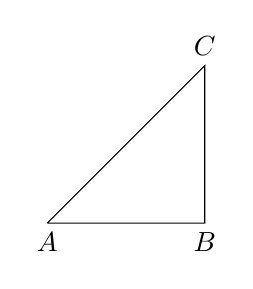
\begin{tikzpicture}
	\draw(0,0)node[below]{$A$}--(2,0)node[below]{$B$}--(2,2)node[above]{$C$}--(0,0);
    \end{tikzpicture}
\end{center}
Sea $\widehat{A}+\widehat{B}+\widehat{C} = 180^{\circ}$. Como $\widehat{B} = 90^{\circ}$, entonces $widehat{A},\widehat{C} < 90^{\circ}$. Luego el ángulo externo a $\widehat{A}$ y $\widehat{C} > 90^{\circ}$ ya que son suplementarios.\\\\

%--------------------5.
\item Notemos que $A\widehat{D}E$ es un ángulo externo al triángulo $DBC$ y por $TAE$ se tiene: $$A\widehat{D}E > D\widehat{B}C, D\widehat{C}B \qquad (1)$$ De la misma manera, $A\widehat{E}C$ es externo a $\triangle ADE$ y una vez más por $TAE$:
$$A\widehat{E}C = A\widehat{D}E \qquad (2),$$ luego por $(2)$ y $(1)$ se tiene que $A\widehat{E}C > D\widehat{B}C$.\\\\ 

%--------------------6.
\item El ángulo $E\widehat{C}D > \widehat{B}, \widehat{A}$ por $TAE$. Como $\triangle ABC = \triangle ECD$ así $E\widehat{C}D=B\widehat{C}A,$ entonces $\overline{AC} = \overline{EC}$ por el teorema de desigualdad triangular tenemos que: $$\overline{AC} + \overline{CB} \geq \overline{AB},$$ como $\overline{AC} = \overline{EC}$ y $\overline{CB} = \overline{CD}$ entonces $$\overline{EC} + \overline{CD} > \overline{AB},$$ luego $\overline{AD} = \overline{AC} + \overline{CD}$ se tiene $$\overline{AD} = \overline{EC} + \overline{CD} > \overline{AB}$$ que implica que $\overline{AD} > \overline{AB}$\\\\

%--------------------7.
\item Simplemente debemos trazar el segmento $AC$ e introducirlo en  $\triangle ADC = \triangle ABC$ según el criterio del catéto de hipotenusa que implica que $AD = BC$.\\\\

%--------------------8.
\item Los triángulos serán congruentes con el caso del caso LAA o con el cateto opuesto.\\\\

%--------------------9.
\item 
\begin{enumerate}[\bfseries a)]
    
    %----------a)
    \item Si son congruentes ya que los ángulos lo son.\\\\ 

    %----------b)
    \item El lado $AB$.\\\\

    %----------c)
    \item El lado $AC$\\\\

\end{enumerate}

%--------------------10.
\item 
\begin{enumerate}[\bfseries a)]
    
    %----------a)
    \item No son congruentes.\\\\

    %----------b)
    \item El lado $AB$.\\\\

    %----------c)
    \item El lado $AC$\\\\

\end{enumerate}




\end{enumerate}


